
\chapter{ಕೆಲವು ವಿಶಿಷ್ಟ ಮಾಯಾಚೌಕಗಳು}

ಮಾಯಾಚೌಕಗಳನ್ನು ಮನರಂಜನೆಗೂ ಬಳಸಬಹುದು. ಅವುಗಳ ರಚನೆಯಲ್ಲಿರುವ ಕೌಶಲ, ಆಕರ್ಷಕ ರೀತಿಯ ವಿನ್ಯಾಸ, ವಿಸ್ಮಯಗೊಳಿಸುವ ಸಂಖ್ಯೆ ಜೋಡಣೆ ಇವು ಮುದ ನೀಡಬಲ್ಲವು. ಕೆಲವನ್ನು ಗಮನಿಸೋಣ.

\section*{VI. 1. ಲೊಸೆ಼ಂಜ್ ಮಾಯಾಚೌಕ :}

ಇದು 5ನೆ ಕ್ರಮವರ್ಗದ ಮಾಯಾಚೌಕವಾದರೂ ಒಂದು ವಿಶಿಷ್ಟತೆ ಇದೆ. $5 \times 5$ ಚೌಕದ \hbox{ನಾಲ್ಕು ಮೂಲೆಗಳಲ್ಲಿ} ಬರುವ ಮೂರು ಮೂರು ಸಂಖ್ಯೆಗಳು ಸಮ ಸಂಖ್ಯೆಗಳು. ನಡುವೆ ಬರುವ ವಜ್ರಾಕೃತಿ ಸದೃಶ ಮನೆಗಳಲ್ಲಿ ಬೆಸ ಸಂಖ್ಯೆಗಳು ಇವೆ.
\begin{figure}[H]
\includegraphics{src/figures/chap5/fig5-1.eps}
\caption*{VI. 1.1 ಮೊತ್ತ : 65}
\end{figure}

\noindent \textbf{ರಚಿಸುವ ಕ್ರಮ :}
\begin{itemize}
	\item $5 \times 5$ ಚೌಕ ರಚಿಸಿ
	\item 4 ಮೂಲೆಗಳಲ್ಲಿ ಹೊರ ಸುತ್ತಿನ 3 ಮನೆಗಳನ್ನು ಬಿಟ್ಟು ಉಳಿದವನ್ನು ಮಸುಕು (shade) ಮಾಡಿ. ವಜ್ರಾಕೃತಿ ಬರುತ್ತದೆ.
	\item ಎಡ ಕಂಭಸಾಲಿನ ಮಧ್ಯದ ಮನೆಯಲ್ಲಿ 1ನ್ನು ಬರೆದು, ಬಲಗಡೆಗೆ ಓರೆಯಾಗಿ ಚಲಿಸುತ್ತಾ ಬೆಸ ಸಂಖ್ಯೆಗಳನ್ನು ತುಂಬಿಸಿ. (1,3,5)
	\item ಮುಂದಿನ ಉಪಕರ್ಣದ ಮನೆಗಳಲ್ಲಿ, ಮುಂದಿನ ಬೆಸ ಸಂಖ್ಯೆಗಳಾದ 7, 9, ತುಂ\-ಬಿಸಿ. ಹೊರ ಆವರಣದ ಮನೆಗಳನ್ನು ತುಂಬಿಸುವುದು ಬೇಡ.
	\item ಹೀಗೆಯೇ 3,2, 3 ಮನೆಗಳಿರುವ ಉಪಕರ್ಣದ ಮನೆಗಳನ್ನು ಕ್ರಮವಾಗಿ ಬೆಸ ಸಂಖ್ಯೆ\-ಗಳಿಂದ ತುಂಬಿಸಿ. ಚಿತ್ರ.VI. 1.1
	\item 1,3,5 ಇರುವ ಉಪಕರ್ಣಕ್ಕೆ ಪೂರಕವಾಗುವ (ಅಂದರೆ 5-3=2) ಎದುರಿಗಿರುವ 2 ಮನೆಗಳಲ್ಲಿ ಇವುಗಳ ನಡುವೆ ಬರಬೇಕಾದ 2, 4 ತುಂಬಿಸಿ.
	\item 4 ಮನೆಗಳ ಉಪಕರ್ಣದ ಮಧ್ಯೆ ಇರುವ 7,9ರ ನಡುವೆ ಬರಬೇಕಾದ 8ನ್ನು ಎದುರಿನ ಮೂಲೆ ಮನೆಯಲ್ಲಿ ತುಂಬಿಸಿ.
	\item ಹೀಗೆಯೇ 17, 19ರ ನಡುವಿನ 18ನ್ನು,21-23-25ಗಳ ನಡುವಿನ 22,24 ಗಳನ್ನು ಎದುರಿನ ಮೂಲೆ ಮನೆಗಳಲ್ಲಿ ತುಂಬಿಸಿ.
	\item ಕರ್ಣದಲ್ಲಿ 11,13,15 ನಡುವೆ ಬರಬೇಕಾದ 12, 14ಗಳನ್ನು ಎದುರು ಮೂಲೆಗಳಲ್ಲಿ ತುಂಬಿಸಿ. ಮಾಯಾಚೌಕ ಸಿದ್ಧ.
\end{itemize}

\section*{VI. 2. ಉಲ್ಟಾ ಪಲ್ಟಾ ಮಾಯಾಚೌಕಗಳು :}

ಕೆಲವು ಮಾಯಾಚೌಕಗಳನ್ನು ತಲೆಕೆಳಗು ಮಾಡಿದಾಗ ಅಂದರೆ $180^\circ$ ಯಷ್ಟು ಸುತ್ತಿಸಿದಾಗ ಮತ್ತೊಂದು ಮಾಯಾಚೌಕ ಲಭಿಸುತ್ತದೆ. ಇವೇ ಉಲ್ಟಾ ಪಲ್ಟಾ ಮಾಯಾಚೌಕಗಳು. ಇವುಗಳಲ್ಲಿ ಬಳಕೆಯಾಗುವ ಅಂಕಿಗಳು ಕೆಲವು ಮಾತ್ರ. ಈ ಉದಾಹರಣೆಗಳನ್ನು ನೋಡಿ.
\begin{figure}[H]
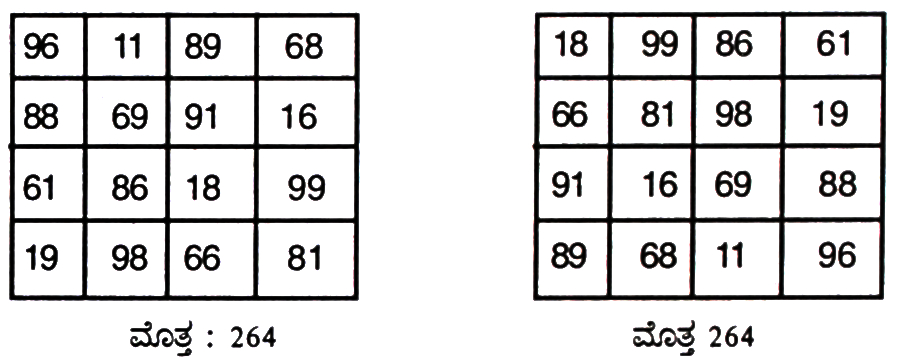
\includegraphics[scale=.9]{src/figures/chap5/fig5-2.jpg}
\end{figure}
\begin{itemize}
	\item 4 ಕ್ರಮವರ್ಗದ ಮಾಯಾಚೌಕ
	\item 1,6,8,9, ಅಂಕಿಗಳನ್ನು ಮಾತ್ರ ಬಳಸಲಾಗಿದೆ.
	\item ಪ್ರತಿಯೊಂದು ಅಡ್ಡಸಾಲು, ಕಂಭಸಾಲು ಮತ್ತು ಕರ್ಣಗಳಲ್ಲಿರುವ ಸಂಖ್ಯೆಗಳ ಏಕಸ್ಥಾನ (unitplace) ಅಂಕಿಗಳನ್ನು ಒಟ್ಟು ಮಾಡಿದರೆ 24 ಬರುತ್ತದೆ.
	\item ಇದೇ ರೀತಿ ಪ್ರತಿ ಸಾಲಿನ ಹತ್ತರ ಸ್ಥಾನದ ಅಂಕಿಗಳ ಮೊತ್ತವೂ 24
	\item ಚೌಕವನ್ನು ನಾಲ್ಕು ಸಮ ಭಾಗಗಳಾಗಿ ವಿಭಾಗಿಸಿದರೆ ಪ್ರತಿ $2 \times 2$ ಚೌಕದ ಸಂಖ್ಯೆಗಳ ಮೊತ್ತ 264
	\item ನಾಲ್ಕು ಮೂಲೆಗಳ ಸಂಖ್ಯೆಗಳ ಮೊತ್ತ 264
	\item ಮಧ್ಯದಲ್ಲಿರುವ $2 \times 2$ಚೌಕದ ಸಂಖ್ಯೆಗಳ ಮೊತ್ತ 264
	\item ಪ್ರತಿಯೊಂದು ಅಡ್ಡಸಾಲು, ಕಂಭಸಾಲು, ಕರ್ಣ - ಇವುಗಳ ಸಂಖ್ಯೆಗಳ ಮೊತ್ತ 264
	\item ಉಪಕರ್ಣಗಳ ಸಂಖ್ಯೆಗಳ ಮೊತ್ತ 264.
\end{itemize}

\section*{VI. 3. ಉಲ್ಟಾ ಪಲ್ಟಾ ಮಾಯಾಚೌಕಕ್ಕೆ ಮತ್ತೊಂದು ಉದಾಹರಣೆ :}

\begin{figure}[H]
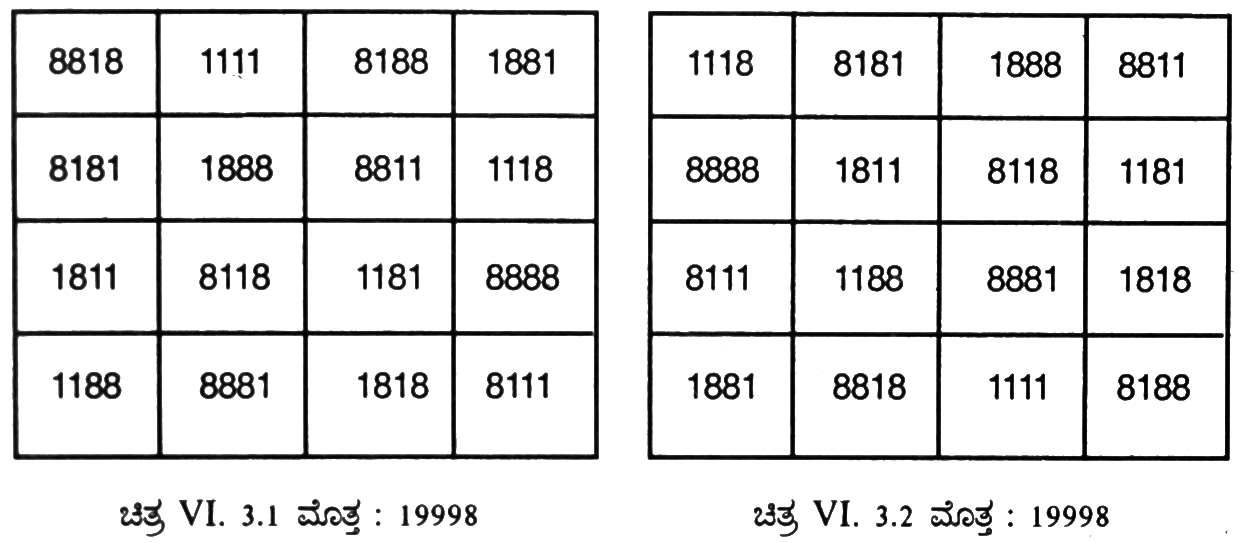
\includegraphics[scale=.9]{src/figures/chap5/fig5-3.jpg}
\end{figure}
\begin{itemize}
	\item ಚೌಕಗಳಲ್ಲಿ 1 ಮತ್ತು 8 ಎರಡು ಅಂಕಿಗಳನ್ನು ಮಾತ್ರ ಬಳಸಿದೆ.
	\item ಚಿತ್ರ VI. 3.1. ಚೌಕವನ್ನು $180^\circ$ ತಿರುಗಿಸಿದರೆ ಚಿತ್ರ VI. 3.2 ಚೌಕ ಲಭ್ಯ
	\item ಪ್ರತಿ ಅಡ್ಡಸಾಲು, ಕಂಭಸಾಲು ಮತ್ತು ಕರ್ಣಗಳ ಸಂಖ್ಯೆಗಳ ಮೊತ್ತ 19998
	\item ನಾಲ್ಕು ಸಮಭಾಗಗಳಾಗಿ ಮಾಡಿದರೆ ಪ್ರತಿ ಭಾಗ $2 \times 2$ ಚೌಕದ ಸಂಖ್ಯೆಗಳ ಮೊತ್ತವೂ 19998
	\item ನಾಲ್ಕು ಮೂಲೆಗಳ ಸಂಖ್ಯೆಗಳ ಮೊತ್ತ 19998
	\item ಮಧ್ಯದ $2 \times 2$ ಚೌಕದ ಸಂಖ್ಯೆಗಳ ಮೊತ್ತ 19998
	\item ಖಂಡ ಕರ್ಣಗಳಲ್ಲಿನ ಸಂಖ್ಯೆಗಳ ಮೊತ್ತ 19998

	ಉದಾ : 8181+1111+8888+1818=19998
	\item ಪ್ರತಿ ಅಡ್ಡಸಾಲು, ಕಂಭಸಾಲು, ಮತ್ತು ಕರ್ಣಗಳಲ್ಲಿನ ಸಂಖ್ಯೆಗಳಲ್ಲಿ ಬಿಡಿ, ಹತ್ತು, \linebreak ನೂರು, ಸಾವಿರ ಸ್ಥಾನದ ಅಂಕಿಗಳ ಮೊತ್ತ 18.
	\item ಈ ಚೌಕಕ್ಕೆ IXOHOXI ಎಂಬ ಹೆಸರಿದೆ.
\end{itemize}
\begin{center}
*****
\end{center}

\section*{VI. 4. ಅವಿಭಾಜ್ಯ ಸಂಖ್ಯೆಗಳಿಂದಾದ ಮಾಯಾಚೌಕಗಳು :}

ಇಂತಹ ಚೌಕಗಳಲ್ಲಿನ ಬಳಸುವ ಎಲ್ಲ ಸಂಖ್ಯೆಗಳೂ ಅವಿಭಾಜ್ಯಸಂಖ್ಯೆಗಳು. (1 ಮತ್ತು ಆ \hbox{ಸಂಖ್ಯೆ ಬಿಟ್ಟರೆ} ಬೇರೆ ಅಪವರ್ತನವಿಲ್ಲದವು) ಇವುಗಳನ್ನು ರಚಿಸುವುದು ಕಷ್ಟಸಾಧ್ಯ. ರಚಿಸಲು ಯಾವುದೇ ನಿರ್ದಿಷ್ಟ ನಿಯಮ ಕಂಡು ಬಂದಿಲ್ಲ. ಒಪ್ಪು -ತಪ್ಪು (trial and error) ವಿಧಾನದಂತೆ ಪ್ರಯತ್ನಿಸಬಹುದು.

ಮಾಯಾಚೌಕಗಳಲ್ಲಿ ಆಸಕ್ತರು ರಚಿಸಿರುವ ಕೆಲವನ್ನು ಪರಿಶೀಲಿಸೋಣ.
\begin{figure}[H]
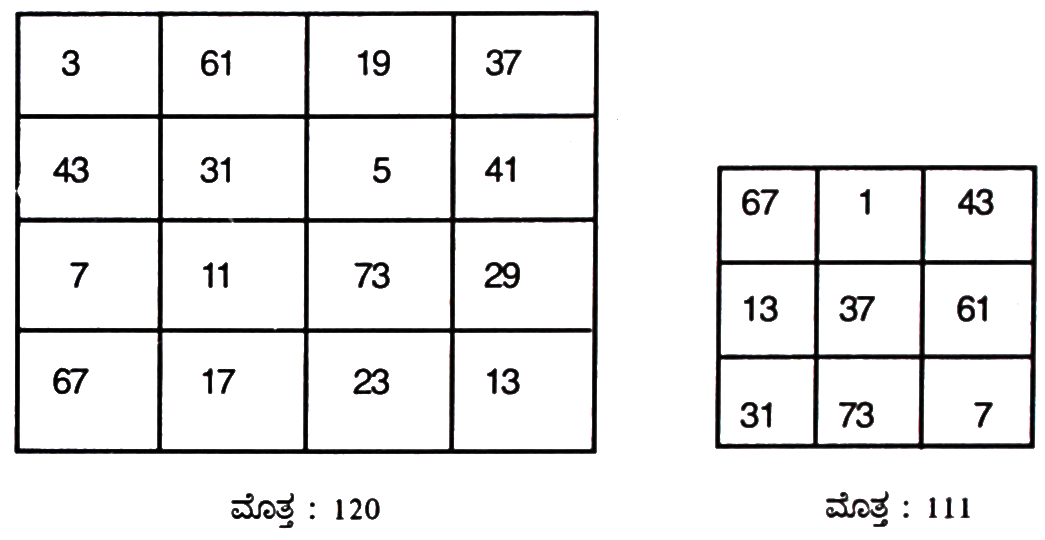
\includegraphics{src/figures/chap5/fig5-4.jpg}
\end{figure}

ಅಮೇರಿಕಾದ ವರ್ಜಿನಿಯಾ ರಾಜ್ಯದ ಅರ್ಲಿಂಗ್ಟನ್ ಎಂಬಲ್ಲಿನ ಆಲನ್ ವಿಲಿಯಂ \hbox{ಜಾನ್ಸನ್} ಎಂಬುವರು 1991ರಲ್ಲಿ 6 ಕ್ರಮವರ್ಗದ ಒಂದು ಮಾಯಾಚೌಕ ರಚಿಸಿ, ಪ್ರಕಟಸಿದ್ದಾರೆ. ಇದರಲ್ಲಿ ಬಳಸಿರುವ ಅವಿಭಾಜ್ಯ. ಸಂಖ್ಯೆಗಳು 67 ರಿಂದ 251 ರ ನಡುವೆ ಬರುತ್ತವೆ. ವಿಶೇಷವೆಂದರೆ ಇದು ಒಂದು ಸರ್ವತೋಮುಖ ಮಾಯಾಚೌಕ.
\begin{figure}[H]
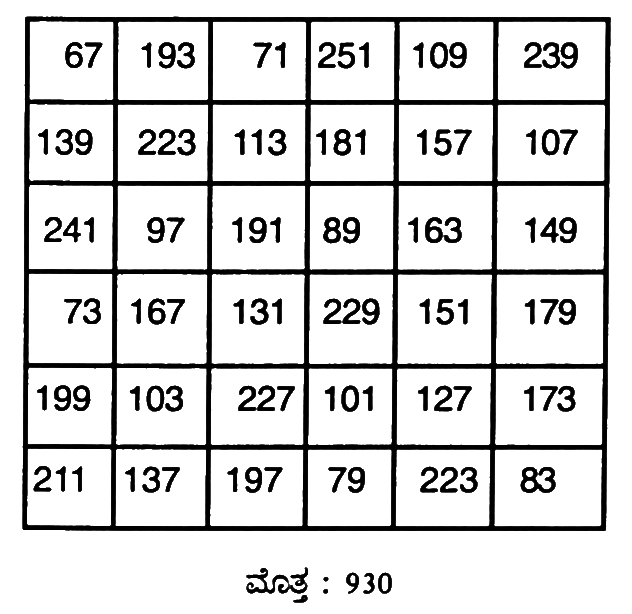
\includegraphics{src/figures/chap5/fig5-5.jpg}
\end{figure}

\textbf{VII. 5.} ಇಂತಹುದೇ ಅವಿಭಾಜ್ಯ ಸಂಖ್ಯೆಗಳಿಂದಾದ ಮತ್ತೊಂದು 7ನೆ ಕ್ರಮವರ್ಗದ ಮಾಯಾಚೌಕವನ್ನು ಗಮನಿಸೋಣ. ಇದರಲ್ಲಿ ಅಡ್ಡಸಾಲು, ಕಂಭಸಾಲು ಮತ್ತು ಕರ್ಣಸಾಲು - ಇವುಗಳ ಸಂಖ್ಯೆಗಳ ಮೊತ್ತ 27627. ಸಮಾಂತರ ಉಪಕರ್ಣಗಳನ್ನು ಅವುಗಳ ಮನೆಗಳ ಸಂಖ್ಯೆ 7 ಆಗುವಂತೆ ತೆಗೆದುಕೊಂಡರೆ, ಆ 7 ಮನೆಗಳಲ್ಲಿನ ಸಂಖ್ಯೆಗಳ ಮೊತ್ತ 27627.

ಇಷ್ಟು ಮಾತ್ರವಲ್ಲ. ಮಾಯಾಚೌಕದ ಎಲ್ಲ 49 ಸಂಖ್ಯೆಗಳಲ್ಲಿಯೂ ಬಿಡಿಸ್ಥಾನ (unitplace)ದ ಅಂಕಿಯನ್ನು ವರ್ಜಿಸಿ (9341 ಎಂಬುದು 934 ಆಗುತ್ತದೆ) ಬರೆದರೆ \hbox{ಲಭಿಸುವ} ಮಾಯಾಚೌಕವೂ ಮೇಲಿನ ಎಲ್ಲ ಲಕ್ಷಣಗಳನ್ನು ಹೊಂದಿರುತ್ತದೆ. ಪರಿಶೀಲಿಸಿ. ಆನಂದಪಡಿ.
\begin{figure}[H]
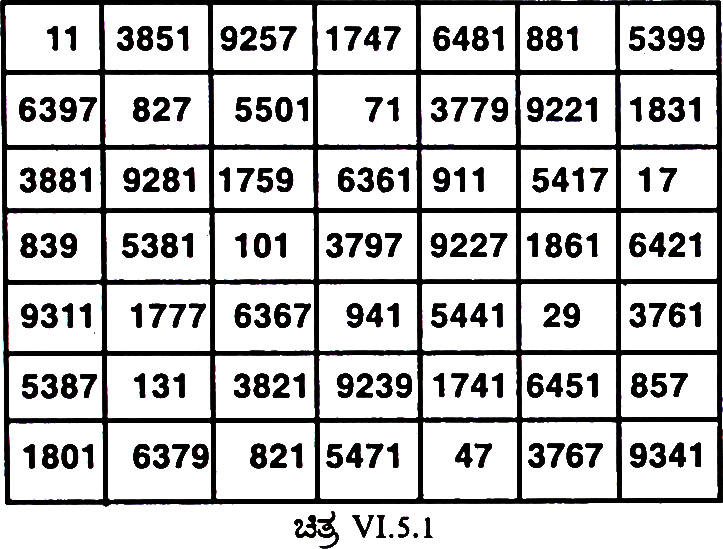
\includegraphics{src/figures/chap5/fig5-6.jpg}
\end{figure}
\begin{itemize}
	\item ಎಲ್ಲ ಸಂಖ್ಯೆಗಳೂ ಅವಿಭಾಜ್ಯ ಸಂಖ್ಯೆಗಳು
	\item ಅಡ್ಡಸಾಲು, ಕಂಭಸಾಲು, ಕರ್ಣಗಳ ಸಂಖ್ಯೆಗಳ ಮೊತ್ತ 27627
	\item ಪೂರಕ ಉಪಕರ್ಣಗಳ ಸಂಖ್ಯೆಗಳ ಮೊತ್ತ 27627
	\begin{figure}[H]
	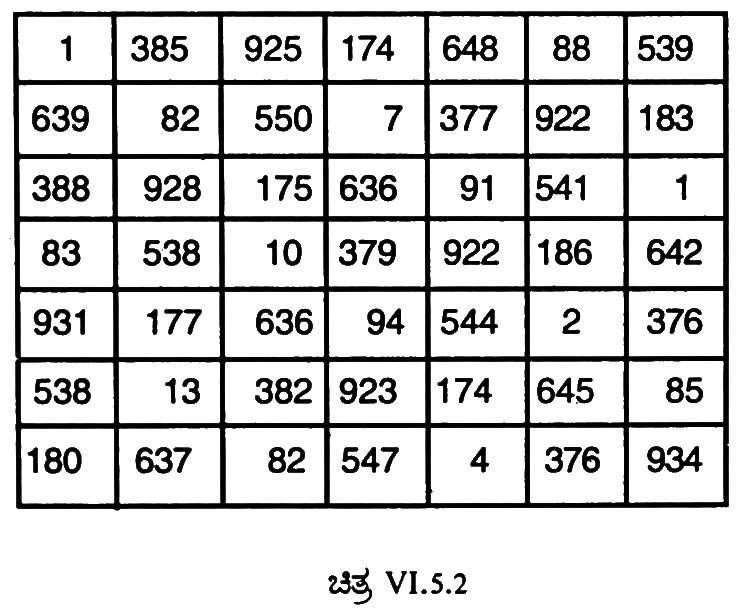
\includegraphics{src/figures/chap5/fig5-7.jpg}
	\end{figure}
	\item ಚಿತ್ರ VI.5.1 ರಲ್ಲಿನ ಸಂಖ್ಯೆಗಳಲ್ಲಿನ ಬಿಡಿಸ್ಥಾನದ ಸಂಖ್ಯೆ ವರ್ಜಿಸಿ ಬರೆದಿದೆ.
	\item ಅಡ್ಡಸಾಲು, ಕಂಭಸಾಲು, ಕರ್ಣಗಳ ಸಂಖ್ಯೆಗಳ ಮೊತ್ತ 2760
	\item ಪೂರಕ ಉಪಕರ್ಣಗಳ ಸಂಖ್ಯೆಗಳ ಮೊತ್ತ 2760
\end{itemize}

\section*{VI. 6. ಆವರಣ ಮಾಯಾಚೌಕ (Bordered Magic Square)}

ಈರುಳ್ಳಿ (ಉಳ್ಳಾಗಡ್ಡೆ) ನೋಡಿದ್ದೀರಲ್ಲ. ಅದರ ಹೊರಗಿನ ಪದರ ತೆಗೆದು ಹಾಕಿದರೆ \linebreak ಸಿಗುವುದೂ ಈರುಳ್ಳಿಯೇ. ಮತ್ತೊಂದು ಪದರ ತೆಗೆದರೂ ಉಳಿಯುವುದು ಈರುಳ್ಳಿಯೇ. ಗಾತ್ರದಲ್ಲಿ ಸ್ವಲ್ಪ ಕಡಿಮೆಯಾಗಬಹುದು ಅಷ್ಟೇ.

ಹೀಗೆಯೇ ಕೆಲವು ಮಾಯಾಚೌಕಗಳಲ್ಲಿಯೂ ಹೊರಸುತ್ತಿನ ಮನೆಗಳಲ್ಲಿನ ಸಂಖ್ಯೆಗಳನ್ನು ವರ್ಜಿಸಿದರೆ ಉಳಿಯುವುದು ಇನ್ನೊಂದು ಮಾಯಾಚೌಕ. ಮತ್ತೆ ಅದರ ಹೊರಸುತ್ತಿನ ಸಂಖ್ಯೆ\-ಗಳನ್ನು ಬಿಟ್ಟರೆ ಉಳಿಯುವುದೂ ಸಹ ಮಾಯಾಚೌಕವೇ. ಇಂತಹ ಮಾಯಾಚೌಕಗಳಿಗೆ \linebreak ಆವರಣ ಮಾಯಾಚೌಕ ಎಂದು ಹೆಸರಿಸಲಾಗಿದೆ. ಉದಾಹರಣೆ ನೋಡಿದರೆ ಸ್ಪಷ್ಟವಾಗ\-ಬಹುದು.
\begin{figure}[H]
\includegraphics[scale=.85]{src/figures/chap5/fig5-8.eps}
\end{figure}
%\begin{figure}[H]
%\includegraphics[scale=.8]{src/figures/chap5/fig5-9.eps}
%\end{figure}

\begin{itemize}
	\item ಚಿತ್ರ VI.6.1 ರಲ್ಲಿ 7 ಕ್ರಮವರ್ಗದ ಮಾಯಾಚೌಕವಿದೆ. ಹೊರಗಿನ ಸುತ್ತನ್ನು \hbox{ಪ್ರತ್ಯೇಕಿಸಲು} ಅದರ ಒಳಗಿನ ಸುತ್ತನ್ನು ಮಸುಕು ಮಾಡಿದೆ.
	\item ಚಿತ್ರ VI.6.2 ರಲ್ಲಿ VI.6.1ರ ಹೊರಗಿನ ಸುತ್ತನ್ನು ಬಿಟ್ಟು $5 \times 5$ಚೌಕ ಬರೆದಿದೆ. ಇದು 5 ಕ್ರಮವರ್ಗದ ಮಾಯಾಚೌಕ.
	\item ಚಿತ್ರ VI.6.3 ರಲ್ಲಿ VI.6.2ರ ಚೌಕದ ಹೊರಸುತ್ತನ್ನು (ಮಸುಕು ಮಾಡಿರು\-ವುದನ್ನ) ವರ್ಜಿಸಿದೆ.ಉಳಿಯುವ $3 \times 3$ ಚೌಕವು 3 ಕ್ರಮವರ್ಗದ ಮಾಯಾಚೌಕ
	\item 1 ರಿಂದ 49 ಸಂಖ್ಯೆ ಬಳಸಿದೆ. ಮಧ್ಯದ ಸಂಖ್ಯೆ 25 ಕೇಂದ್ರ ಮನೆಯಲ್ಲಿದೆ. ಅದರ ಸುತ್ತಲೂ ಎದುರು ಮನೆಗಳಲ್ಲಿನ ಸಮಾನ ದೂರದ ಸಂಖ್ಯೆಗಳ ಮೊತ್ತ 50 ಗಮನಿಸಿ. ಆವರಣ ಮಾಯಾಚೌಕಕ್ಕೆ ಮತ್ತೊಂದು ಉದಾಹರಣೆ ನೋಡಿ.
	\begin{figure}[H]
	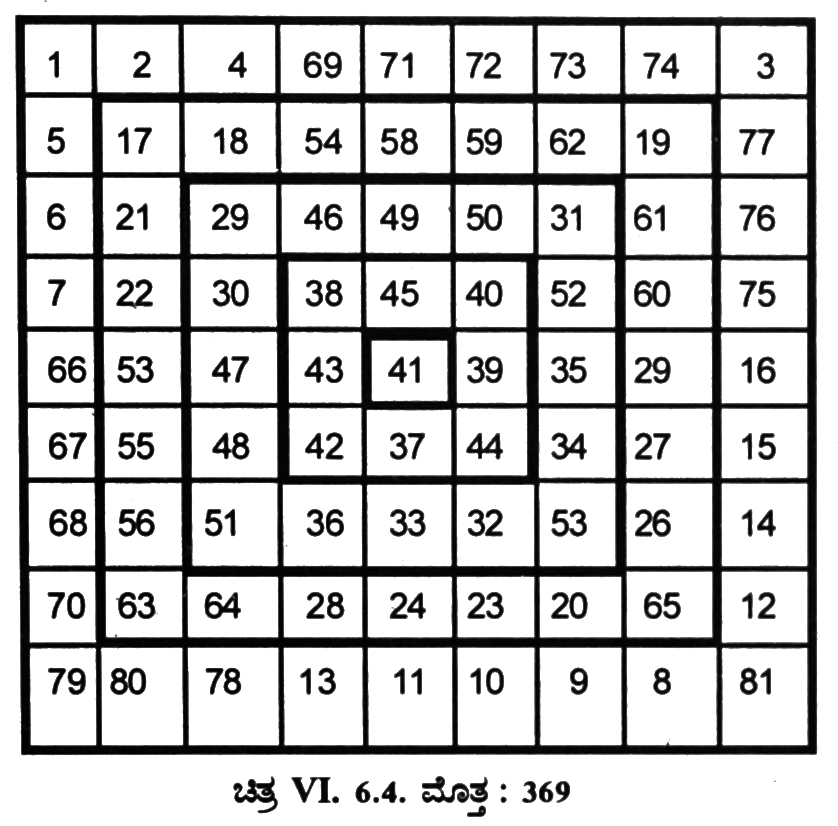
\includegraphics[scale=.9]{src/figures/chap5/fig5-10.jpg}
	\end{figure}
	\begin{figure}[H]
	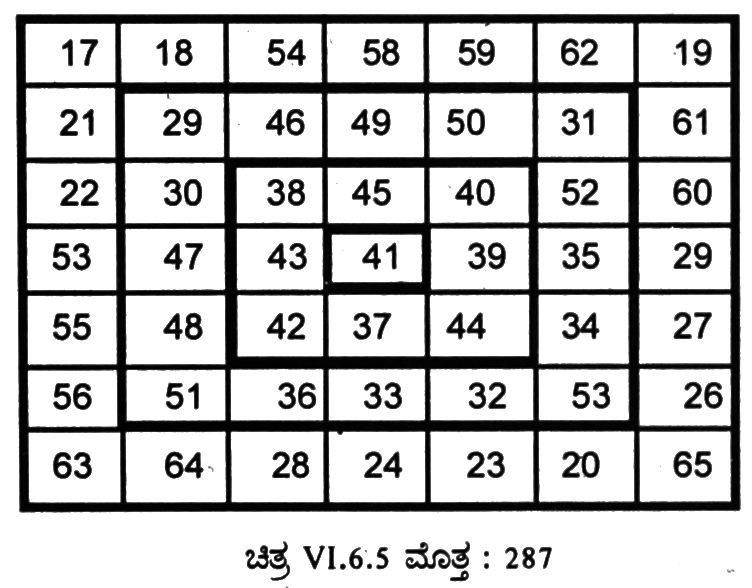
\includegraphics[scale=.9]{src/figures/chap5/fig5-11.jpg}
	\end{figure}
	\begin{figure}[H]
	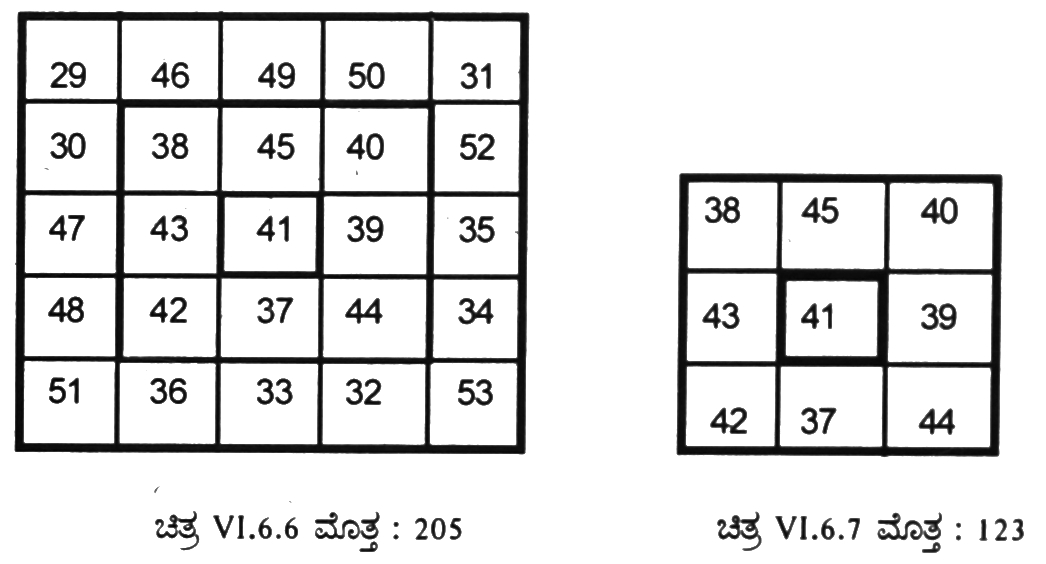
\includegraphics[scale=.9]{src/figures/chap5/fig5-12.jpg}
	\end{figure}

	\item ಚಿತ್ರ VI.6.4ರಲ್ಲಿ $9 \times 9$ಮಾಯಾಚೌಕವಿದೆ. ಇದರ ಹೊರ ಆವರಣ ಬಿಟ್ಟರೆ $7 \times 7$ಚೌಕ ಬರುತ್ತದೆ. ಚಿತ್ರ VI. 6.5 ಇದೂ ಮಾಯಾಚೌಕ. ಇದರ ಹೊರ ಆವರಣ ವರ್ಜಿಸಿದಾಗ $5 \times 5$ಚೌಕ ಲಭಿಸುತ್ತದೆ. ಚಿತ್ರ VI. 6.6 ಇದೂ ಮಾಯಾ ಚೌಕ. ಇದರ ಹೊರ ಆವರಣ ತೆಗೆದು ಹಾಕಿದರೆ $3 \times 3$ಚೌಕ ದೊರೆಯುತ್ತದೆ. ಇದೂ ಸಹ ಮಾಯಾಚೌಕ.
	\item ಪ್ರತಿ ಮಾಯಾಚೌಕದಲ್ಲಿಯೂ ಕೇಂದ್ರ ಸಂಖ್ಯೆ 41. ಕರ್ಣಗಳು, ಅಡ್ಡಸಾಲು, \hbox{ಕಂಭಸಾಲುಗಳಲ್ಲಿ} 41ರಿಂದ ಸಮಾನದೂರದಲ್ಲಿರುವ ಜೋಡಿಸಂಖ್ಯೆಗಳ ಮೊತ್ತ 82. (40+42,53+29) ಉಳಿದ ಅಡ್ಡಸಾಲು, ಕಂಭಸಾಲುಗಳಲ್ಲಿ ತುದಿಯಲ್ಲಿನ ಜೋಡಿ ಸಂಖ್ಯೆಗಳ ಮೊತ್ತ 82 (18+64,50+32, 48+34, 22+60)ಇತ್ಯಾದಿ.
\end{itemize}

\section*{VI. 7. ಮಾಲಾಸಂಖ್ಯೆಗಳಿಂದಾದ ಮಾಯಾಚೌಕ :}

ಕೆಲವು ಸಂಖ್ಯೆಗಳನ್ನು ಹಿಂದು ಮುಂದಾಗಿ ಓದಿದರೂ ಅದೇ ಆಗಿರುತ್ತದೆ. ಉದಾ : 252. ಇಂತಹ ಸಂಖ್ಯೆಗಳಿಗೆ \textbf{‘‘ಮಾಲಾಸಂಖ್ಯೆ’’} ಗಳೆಂದು ಹೆಸರು. (Palindrome Numbers) ಮಾಲಾ ಪದಗಳಿವೆ ಎಂಬುದನ್ನು ನೆನಪಿಸಿಕೊಳ್ಳಿ. ಜಲಜ, ಚಮಚ, ನವವನ, ವಿಕಟಕವಿ ಇವು ಕೆಲವು ಉದಾಹರಣೆಗಳು.

ಫ್ರೆಂಚ್ ಗಣಿತಜ್ಞೆ ಸೋಫಿ ಜರ್ಮೇನ್ 1776ರಲ್ಲಿ ರಚಿಸಿದ ಎರಡು ಮಾಯಾಚೌಕಗಳನ್ನು (3 ಕ್ರಮವರ್ಗ)ಇಲ್ಲಿ ಕೊಡಲಾಗಿದೆ. ಎಲ್ಲ ಸಂಖ್ಯೆಗಳೂ ಮಾಲಾ ಸಂಖ್ಯೆಗಳೇ. ಚಿತ್ರ VI.7.2 ರಲ್ಲಿರುವ ಚೌಕದ ಸಂಖ್ಯೆಗಳು, ಚಿತ್ರ VI. 7.1 ರ ಸಂಖ್ಯೆಗಳ $2n+1$ ಆಗಿವೆ. ಉದಾ : $505=252 \times 2+1$
\begin{figure}[H]
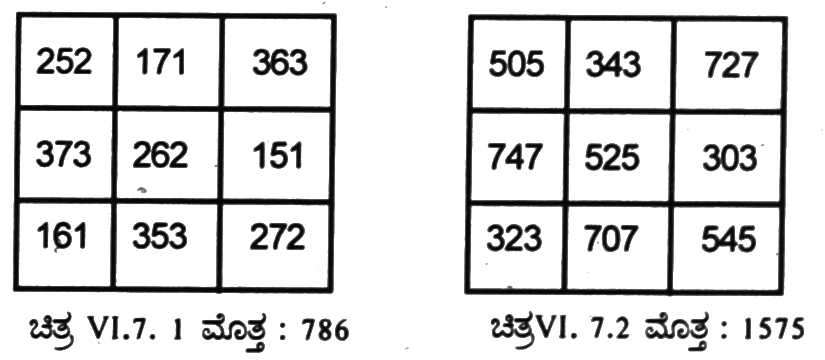
\includegraphics{src/figures/chap5/fig5-13.jpg}
\end{figure}

ಸಂಖ್ಯಾಲೋಕದಲ್ಲಿ ವಿಹರಿಸಿ ಆನಂದ ಪಡೆಯುವುದು ಕೆಲವು ಗಣಿತಜ್ಞರ ಆಸಕ್ತಿ. ಕೆಲವೊಮ್ಮೆ ವಿಶಿಷ್ಟ ವಿಚಿತ್ರ ಫಲಿತಗಳು ದೊರೆಯುವುದೂ ಉಂಟು. ಶ್ರೀನಿವಾಸ ರಾಮಾನುಜರು ಇಂತಹ ಆಸಕ್ತಿಗೆ ಶ್ರೇಷ್ಠ ಉದಾಹರಣೆ. ಅವರ ಹೆಸರಿನಲ್ಲಿರುವ ಸಂಖ್ಯೆ 1729ರ ಬಗೆಗೆ ತಿಳಿದು ನೋಡಿ.

ಮಾಯಾಚೌಕಗಳೂ ಮತ್ತು ಸಂಖ್ಯೆಗಳು ಎರಡರಲ್ಲೂ ಪ್ರಯೋಗಗಳನ್ನು ನಡೆಸಿ, ಉತ್ತಮ ಫಲಿತಾಂಶಗಳನ್ನು ಗಳಿಸಿದ್ದಾರೆ ಕೆಲವು ಗಣಿತಜ್ಞರು, ಈ ಕೆಳಗೆ ಅಂತಹ ಎರಡು ಮಾಯಾಚೌಕ\-ಗಳನ್ನು ಕೊಟ್ಟಿದೆ. ಒಂದು ಆವರಣ ಮಾಯಾಚೌಕ. ಇನ್ನೊಂದು ಗುಚ್ಛ ಮಾಯಾಚೌಕ. \hbox{ಎರಡರಲ್ಲಿ ಬಳಸಿರುವ} ಎಲ್ಲ ಸಂಖ್ಯೆಗಳೂ ಮಾಲಾಸಂಖ್ಯೆಗಳೇ.

\section*{ಆವರಣ ಮಾಯಾಚೌಕ :}

\begin{figure}[H]
\includegraphics{src/figures/chap5/fig5-14.eps}
\end{figure}

\begin{itemize}
	\item 8 ಕ್ರಮವರ್ಗದ ಮಾಯಾಚೌಕ.
	\item ಎಲ್ಲ ಮಾಲಾ ಸಂಖ್ಯೆಗಳು (ತಿರುವು ಮುರುವು ಮಾಡಿದರೂ ಅದೇ ಸಂಖ್ಯೆ. Palindrome Numbers)
	\item ಆವರಣ ಮಾಯಾಚೌಕ
	\item ಹೊರಗಿನ ಒಂದುಸುತ್ತು ಸಂಖ್ಯೆಗಳನ್ನುವಿಸರ್ಜಿಸಿದರೆ 6 ಕ್ರಮವರ್ಗದ ಮಾಯಾಚೌಕ ಲಭ್ಯ
	\item ಇದರ ಹೊರಸುತ್ತಿನ ಸಂಖ್ಯೆಗಳನ್ನು ಕಳಚಿ ಹಾಕಿದಾಗ ಉಳಿಯುವುದು 4 ಕ್ರಮ\-ವರ್ಗದ ಮಾಯಾಚೌಕ.
	\item $8 \times 8$ ಚೌಕ ಮೊತ್ತ 4884, $6 \times 6$ ಚೌಕ ಮೊತ್ತ 3663, $4 \times 4$ ಚೌಕ ಮೊತ್ತ 2442 ಮೊತ್ತ ಸಂಖ್ಯೆಗಳೂ ಮಾಲಾ ಸಂಖ್ಯೆಗಳು.
\end{itemize}

\section*{ಗುಚ್ಛ ಮಾಯಾಚೌಕ :}

\begin{figure}[H]
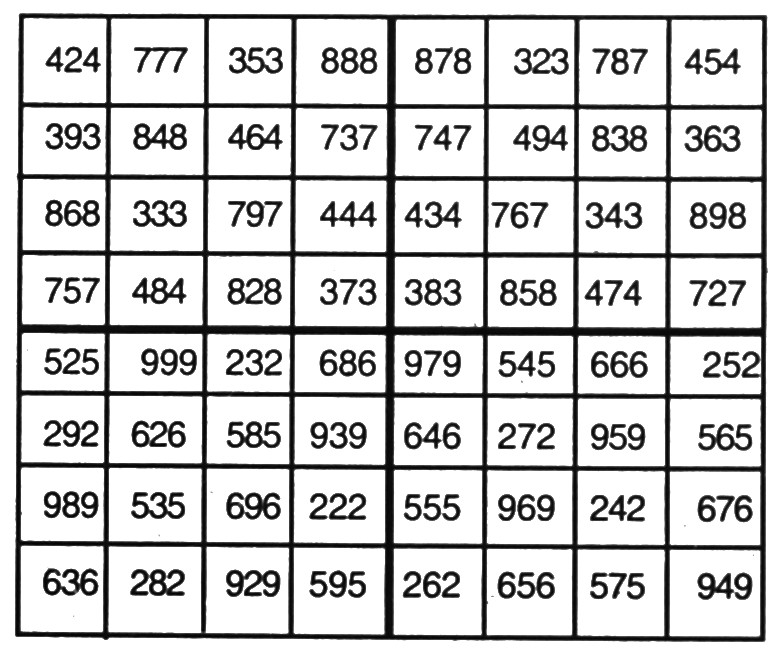
\includegraphics{src/figures/chap5/fig5-15.jpg}
\end{figure}

\begin{itemize}
	\item 8 ಕ್ರಮವರ್ಗದ ಮಾಯಾಚೌಕ.
	\item ಎಲ್ಲ ಮಾಲಾಸಂಖ್ಯೆಗಳು
	\item ಗುಚ್ಛ ಮಾಯಾಚೌಕ. $4 \times 4$ ರ ನಾಲ್ಕು ಚೌಕಗಳಿವೆ.
	\item ಮೊತ್ತ 4884
	\item $4 \times 4$ ಭಾಗಗಳ ಮೊತ್ತ ಪ್ರತಿಯೊಂದೂ 2442
\end{itemize}
\begin{center}
*****
\end{center}
